\appendix
\chapter{Hexagonal country boundaries}
\label{ch:appendix_a}
	\begin{figure}[ht]
		\centering
		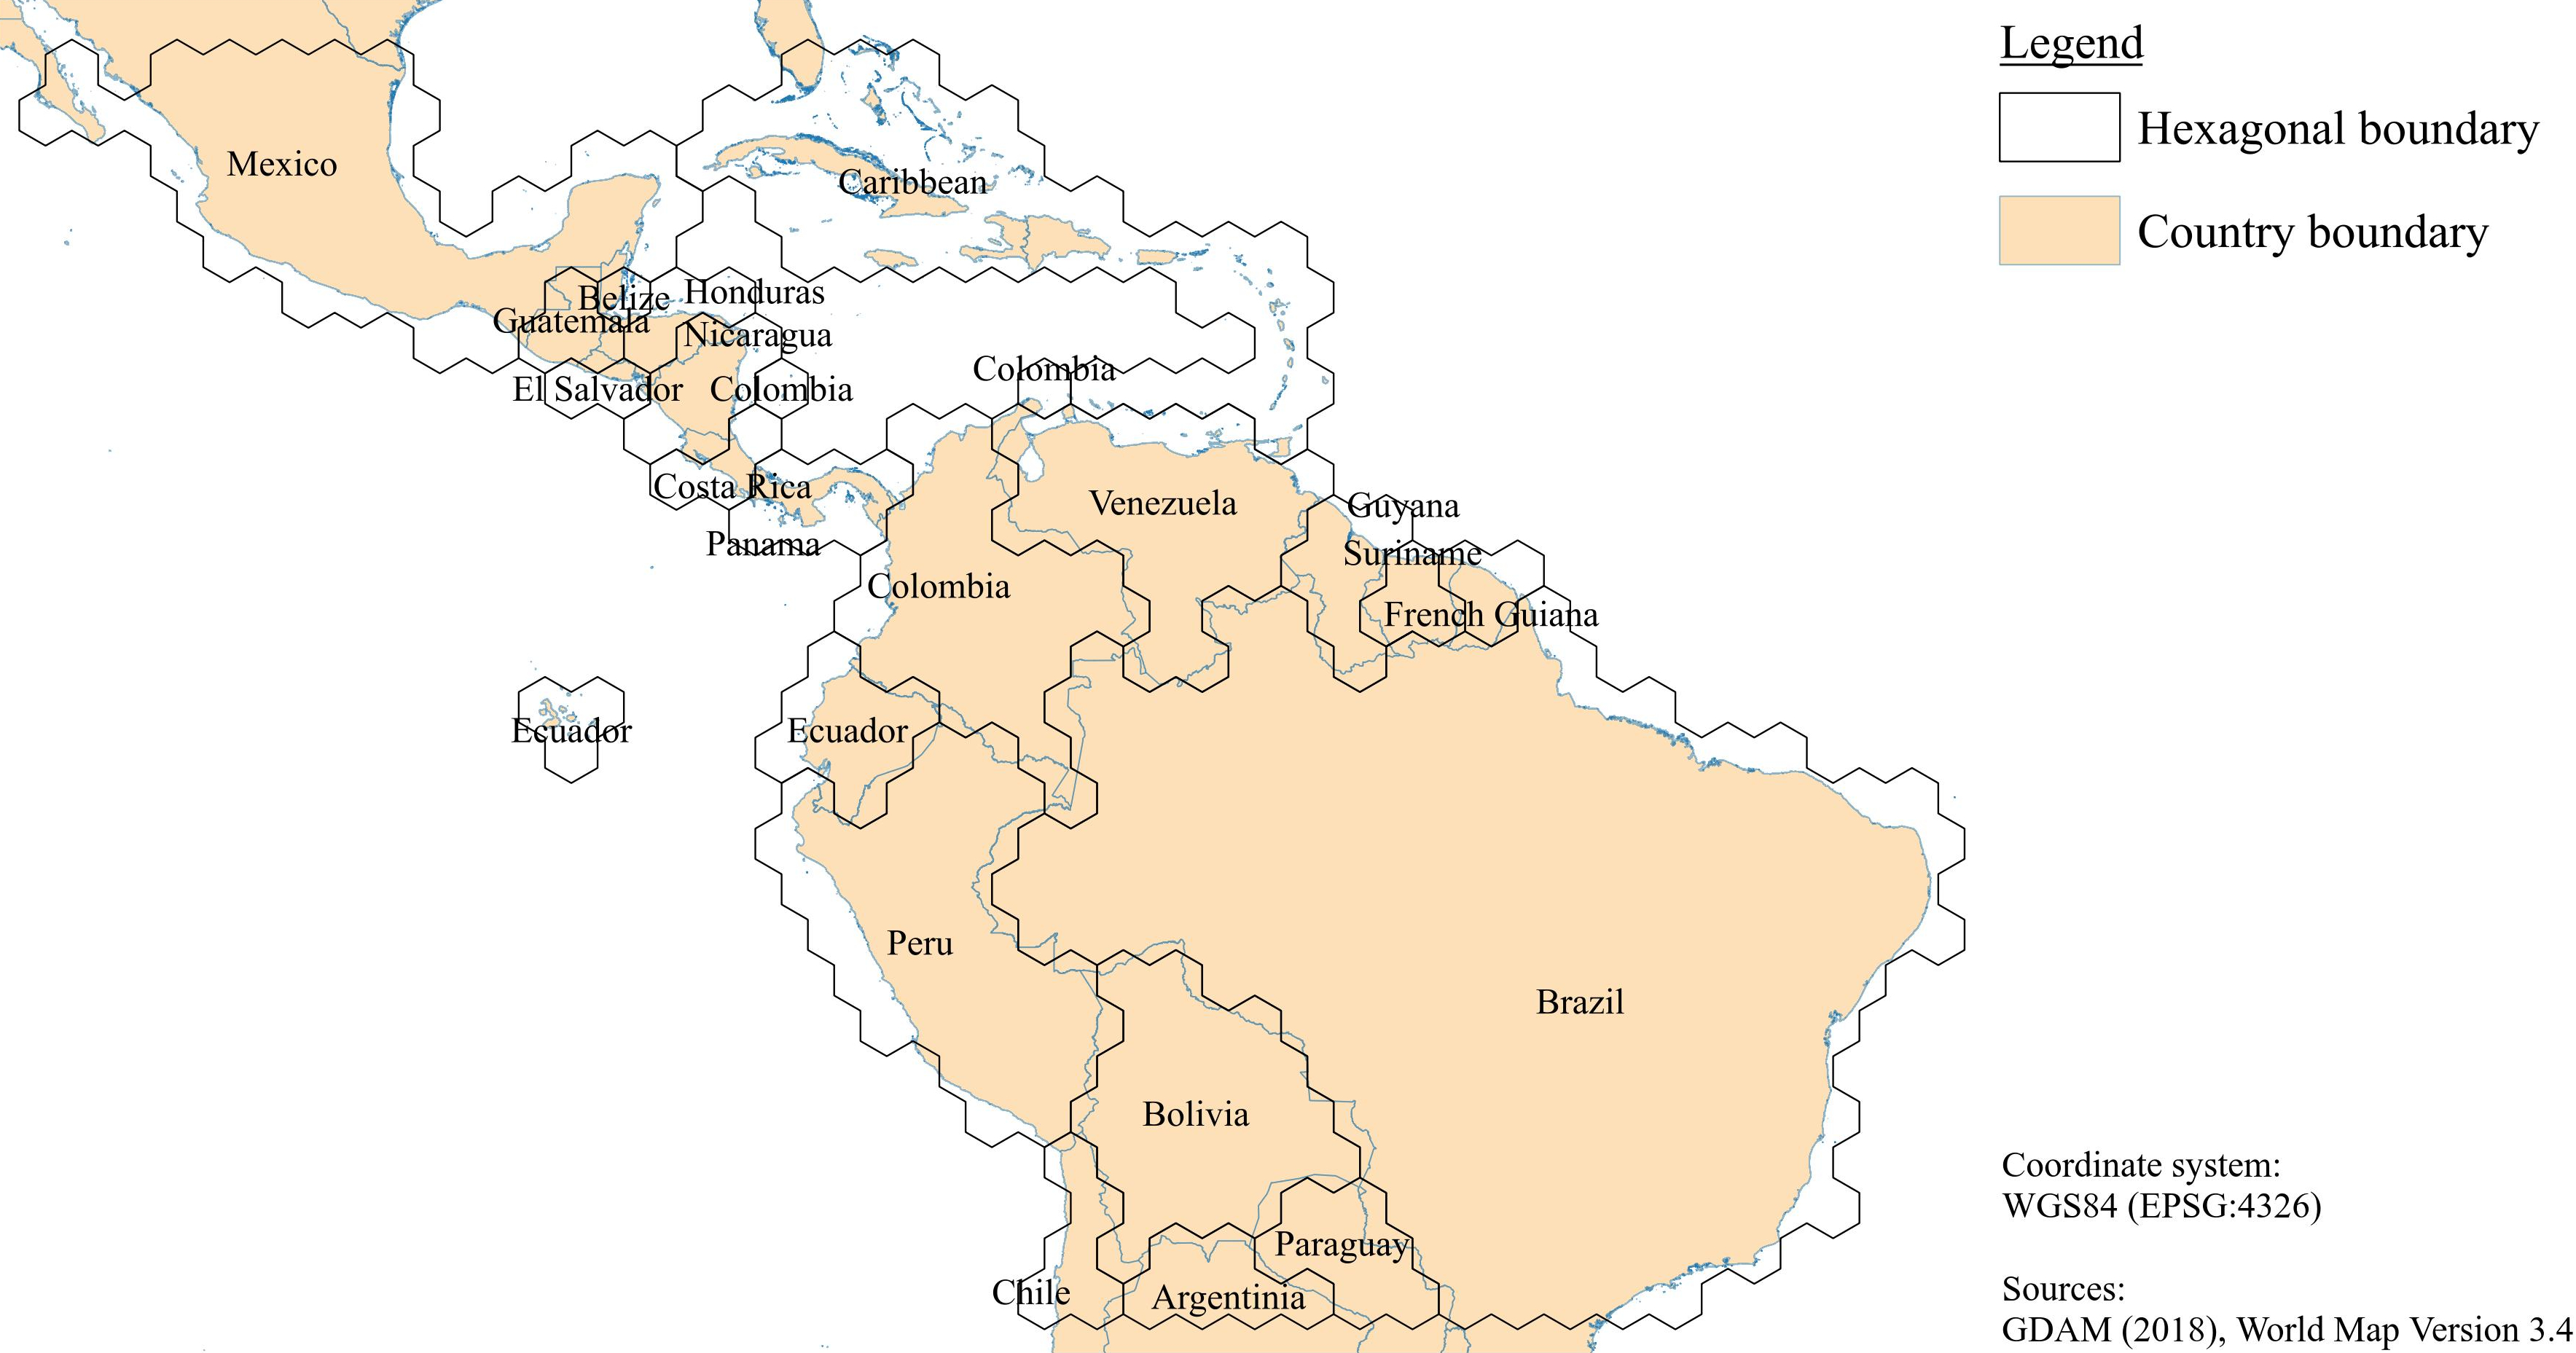
\includegraphics[scale=1.]{img/americas_hexagonal_boundaries}
		\caption[Map of Latin America and its countries]{\textbf{Map of Latin America and its countries:} A}
		\label{fig:americas_hexagonal_appendix}
	\end{figure}
	\begin{figure}[ht]
		\centering
		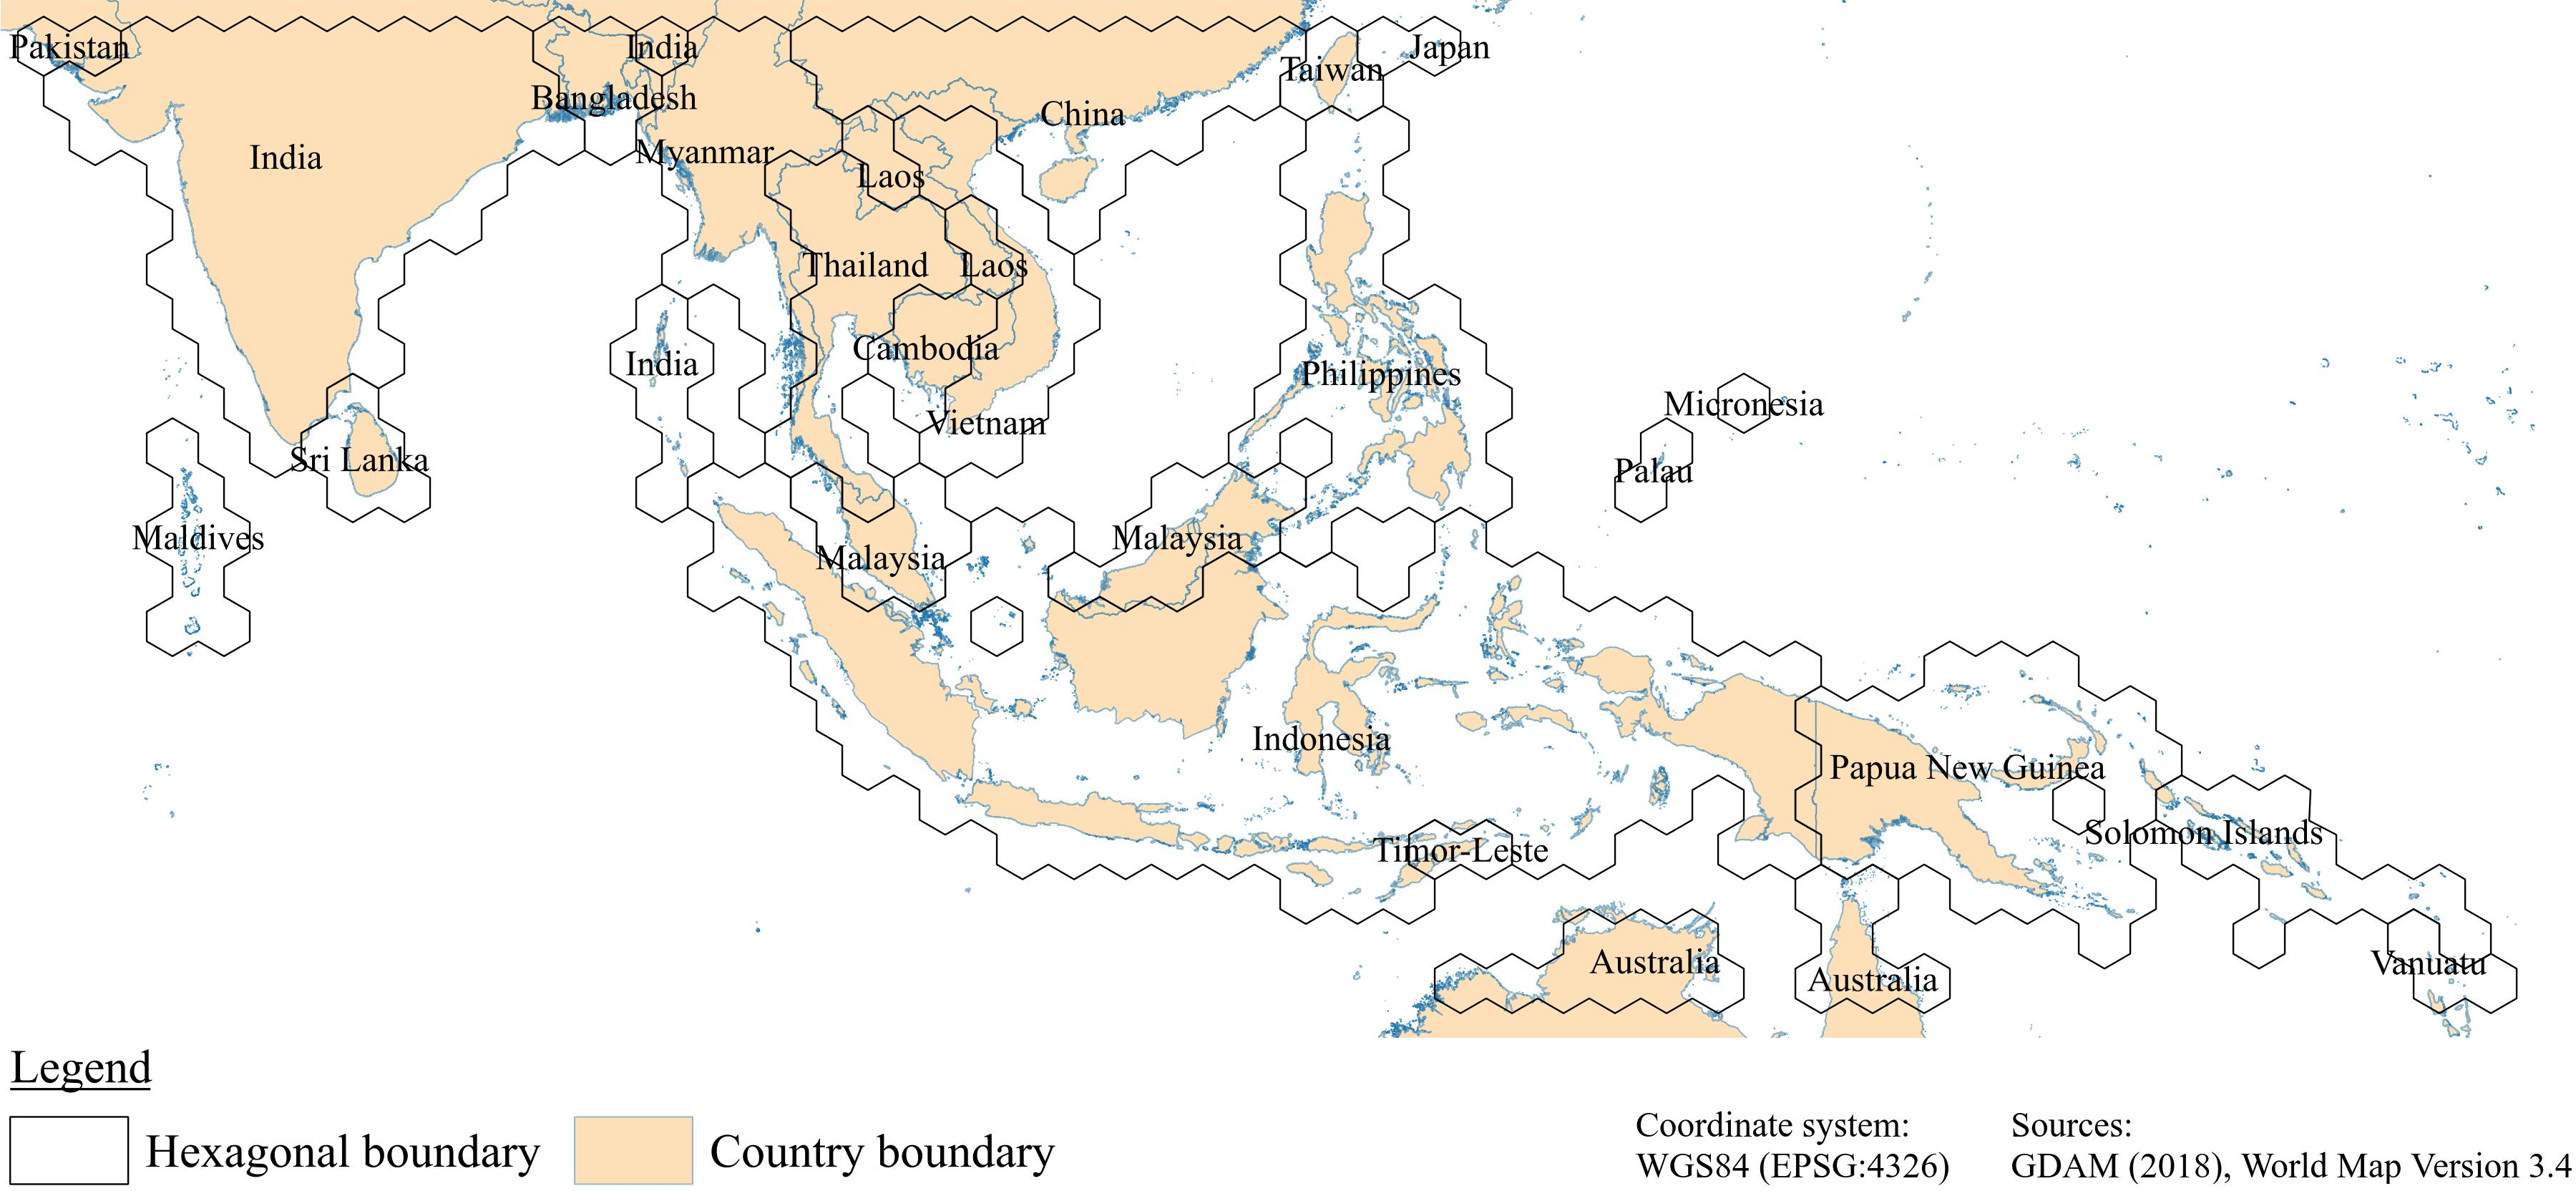
\includegraphics[scale=1.]{img/asia_hexagonal_boundaries}
		\caption[Map of Asia/Australia and its countries]{\textbf{Map of Asia/Australia and its countries:} A}
		\label{fig:asia_hexagonal_appendix}
	\end{figure}
	\begin{figure}[t]
		\centering
		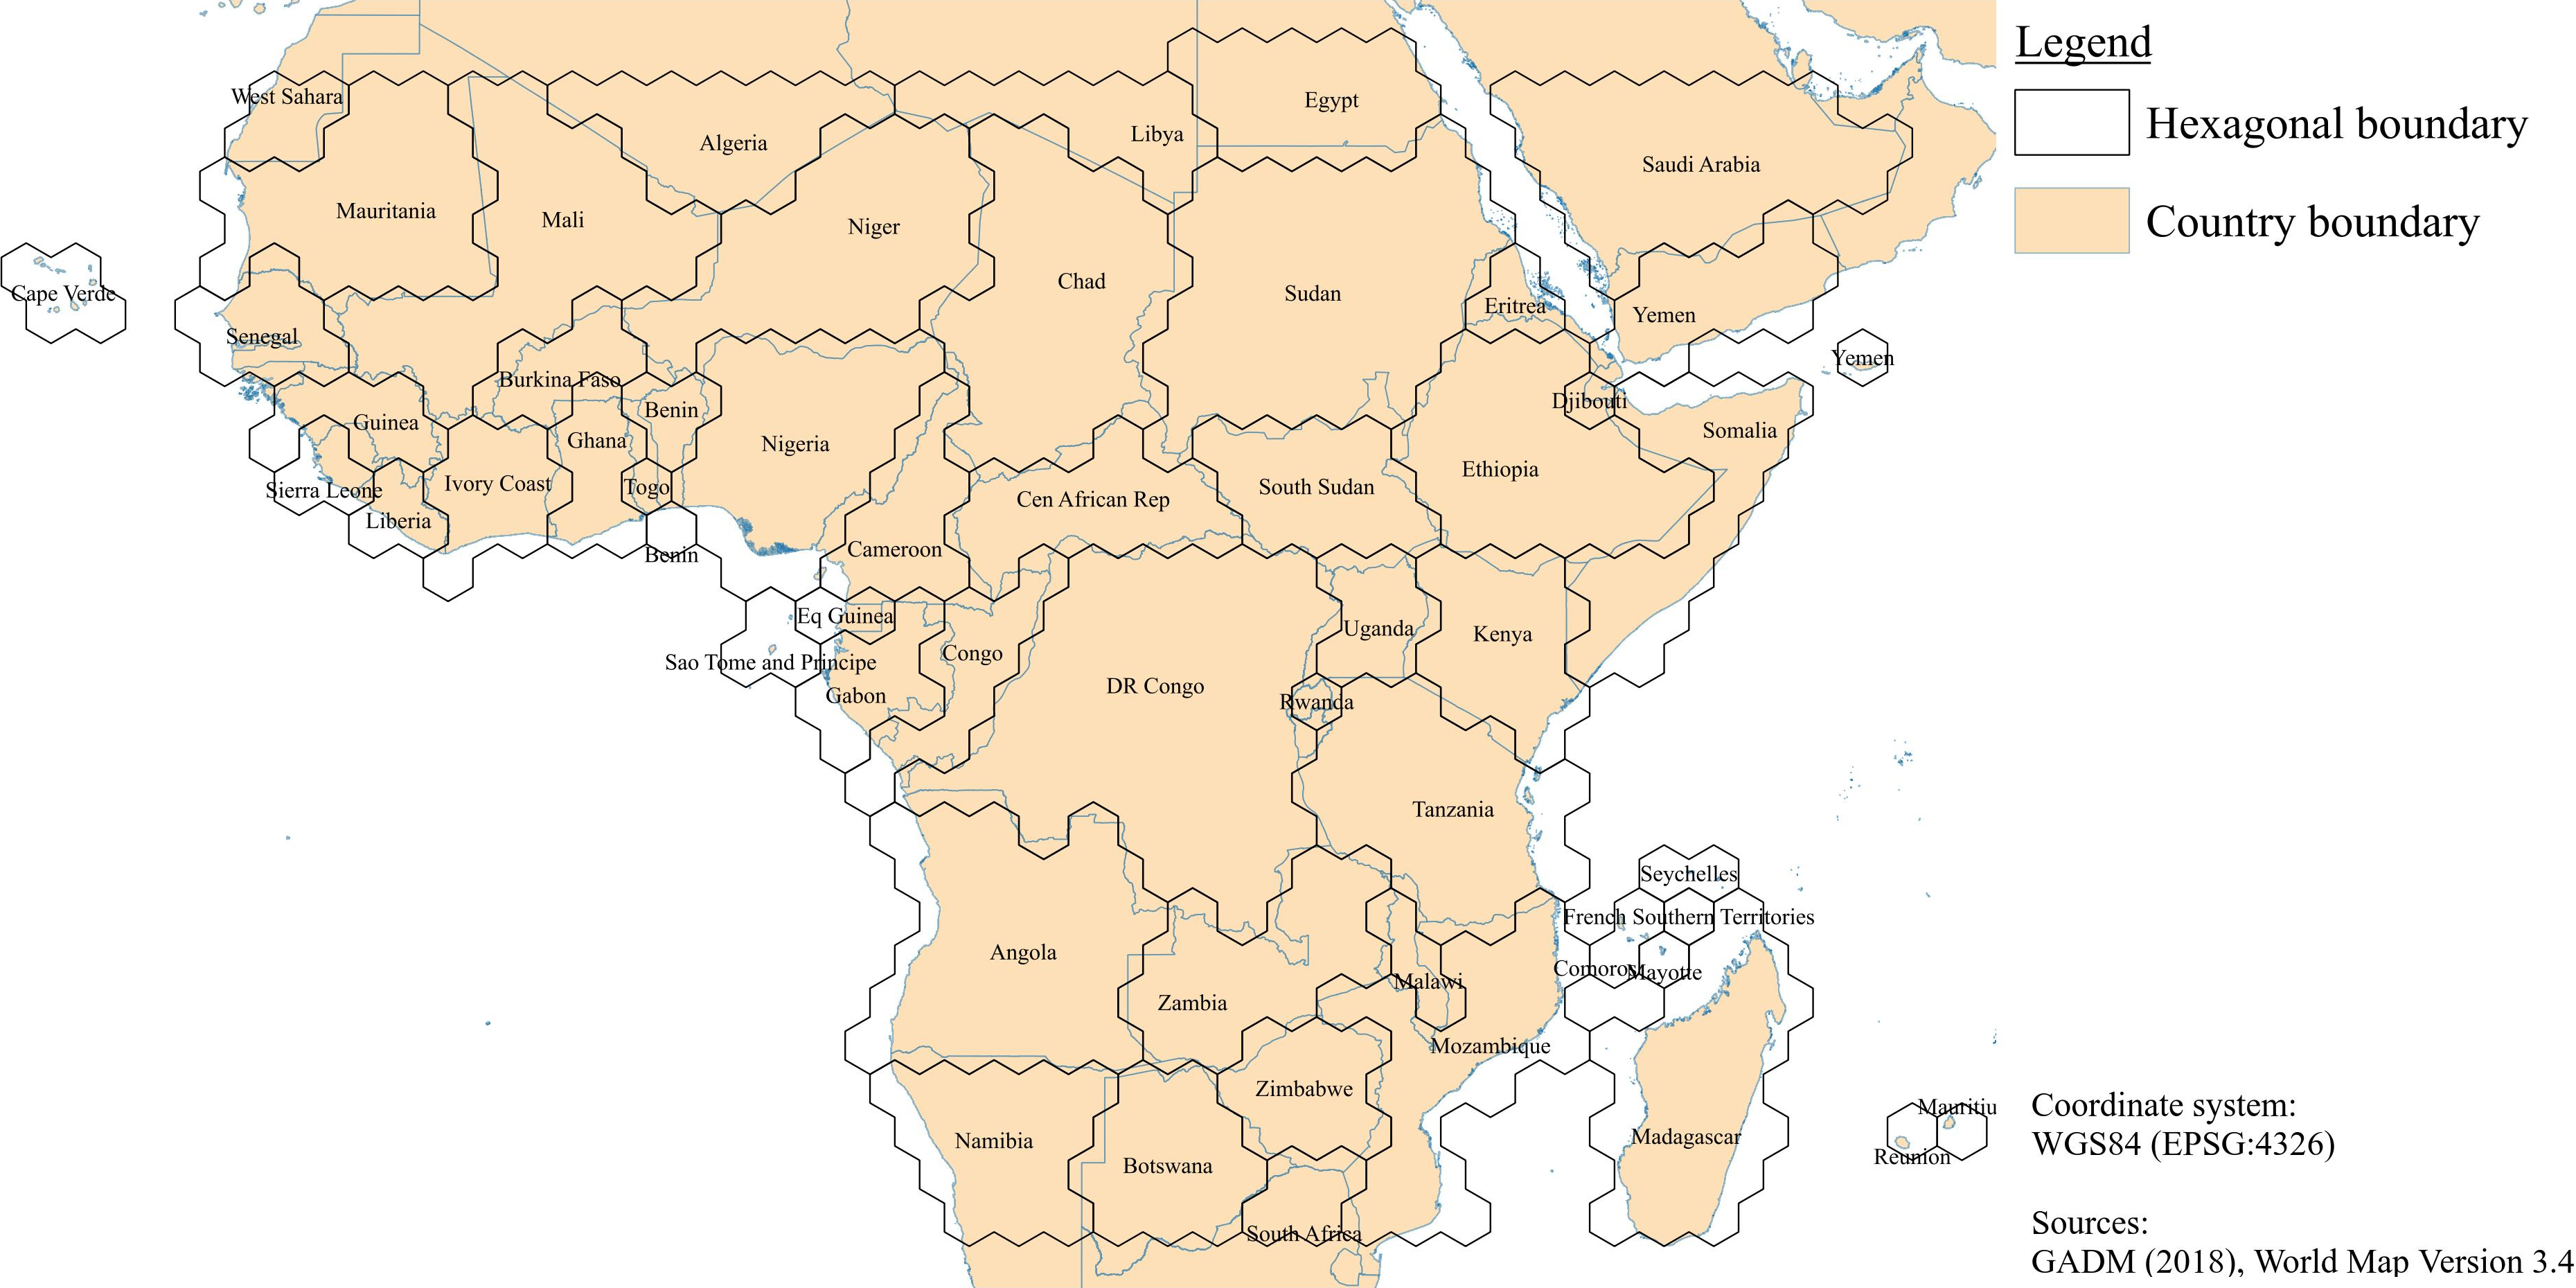
\includegraphics[scale=.98]{img/africa_hexagonal_boundaries}
		\caption[Map of Africa and its countries]{\textbf{Map of Africa and its countries:} A}
		\label{fig:africa_hexagonal_appendix}
	\end{figure}

\chapter{Forest definition}
\label{ch:appendix_b}
%TODO images: captions
	\begin{table}[ht]
		\centering
		\caption[Comparison of tree cover agreement between regions]{\textbf{Comparison of tree cover agreement between regions:} This table shows, a comparison of tree cover agreement between regions. The classes $JI_0$, $JI_1$, $JI_2$, and $JI_3$ as row and column headings account for the canopy density classes (0,100], (10,100], (20,100], and (30,100], respectively. The test hypothesis is H$_0$: $X_1=X_2$ where $X_1$ is the column $JI_n$ class and $X_2$ the row $JI_n$ class. The significance is indicated by $p^{*}<0.05$, $p^{**}<0.02$, and $p^{***}<0.01$. We applied a Benjamini and Hochberg correction for multiple-pairwise testing.}
		\label{tab:wilcoxononesided_comparison}
		\begin{tabular}{llllllllll}
			\hline
			& & \multicolumn{4}{|c}{Latin America} & \multicolumn{4}{|c|}{Asia/Australia} \\
			& Cls & JI$_0$ & JI$_1$ & JI$_2$ & JI$_3$ & JI$_0$ & JI$_1$ & JI$_2$ & JI$_3$ \\\hline
			\multirow{4}{*}{\STAB{\rotatebox[origin=c]{90}{Asia}}}
			& JI$_0$ & .04$^{*}$ & - & - & - & - & - & - & - \\
			& JI$_1$ & - & .04$^{*}$ & - & - & - & - & - & - \\
			& JI$_2$ & - & - & .05$^{*}$ & - & - & - & - & - \\
			& JI$_3$ & - & - & - & .07 & - & - & - & - \\\cline{1-1}
			\multirow{4}{*}{\STAB{\rotatebox[origin=c]{90}{Africa}}} 
			& JI$_0$ & .00$^{***}$ & - & - & - & .00$^{***}$ & - & - & - \\
			& JI$_1$ & - & .00$^{***}$ & - & - & - & .00$^{***}$ & - & - \\
			& JI$_2$ & - & - & .00$^{***}$ & - & - & - & .00$^{***}$ & - \\
			& JI$_3$ & - & - & - & .00$^{***}$ & - & - & - & .00$^{***}$ \\\hline
		\end{tabular}
	\end{table}
	\begin{table}[ht]
		\centering
		\caption[Comparison of tree cover agreement between regions]{\textbf{Comparison of tree cover agreement between regions:} This table shows, a comparison of tree cover agreement between regions and the direction of differences. The classes $JI_0$, $JI_1$, $JI_2$, and $JI_3$ as row and column headings account for the canopy density classes (0,100], (10,100], (20,100], and (30,100], respectively. The test hypothesis is H$_0$: $X_1\leq X_2$ where $X_1$ is the column $JI_n$ class and $X_2$ the row $JI_n$ class. The significance is indicated by $p^{*}<0.05$, $p^{**}<0.025$, $p^{***}<0.01$, and $p^{\dagger}<0.005$. We applied a Benjamini and Hochberg correction for multiple-pairwise testing.}
		\label{tab:wilcoxontwosided_comparison}
		\begin{tabular}{llllllllll}
			\hline
			& & \multicolumn{4}{|c}{Latin America} & \multicolumn{4}{|c|}{Asia/Australia} \\
			& Cls & JI$_0$ & JI$_1$ & JI$_2$ & JI$_3$ & JI$_0$ & JI$_1$ & JI$_2$ & JI$_3$ \\\hline
			\multirow{4}{*}{\STAB{\rotatebox[origin=c]{90}{Asia}}}
			& JI$_0$ & 1. & - & - & - & - & - & - & - \\
			& JI$_1$ & - & 1. & - & - & - & - & - & - \\
			& JI$_2$ & - & - & 1. & - & - & - & - & - \\
			& JI$_3$ & - & - & - & 1. & - & - & - & - \\\cline{1-1}
			\multirow{4}{*}{\STAB{\rotatebox[origin=c]{90}{Africa}}} 
			& JI$_0$ & .00$^{\dagger}$ & - & - & - & .00$^{\dagger}$ & - & - & - \\
			& JI$_1$ & - & .00$^{\dagger}$ & - & - & - & .00$^{\dagger}$ & - & - \\
			& JI$_2$ & - & - & .00$^{\dagger}$ & - & - & - & .00$^{\dagger}$ & - \\
			& JI$_3$ & - & - & - & .00$^{\dagger}$ & - & - & - & .00$^{\dagger}$ \\\hline
		\end{tabular}
	\end{table}

	\begin{landscape}
		\begin{figure}[ht]
				\centering
				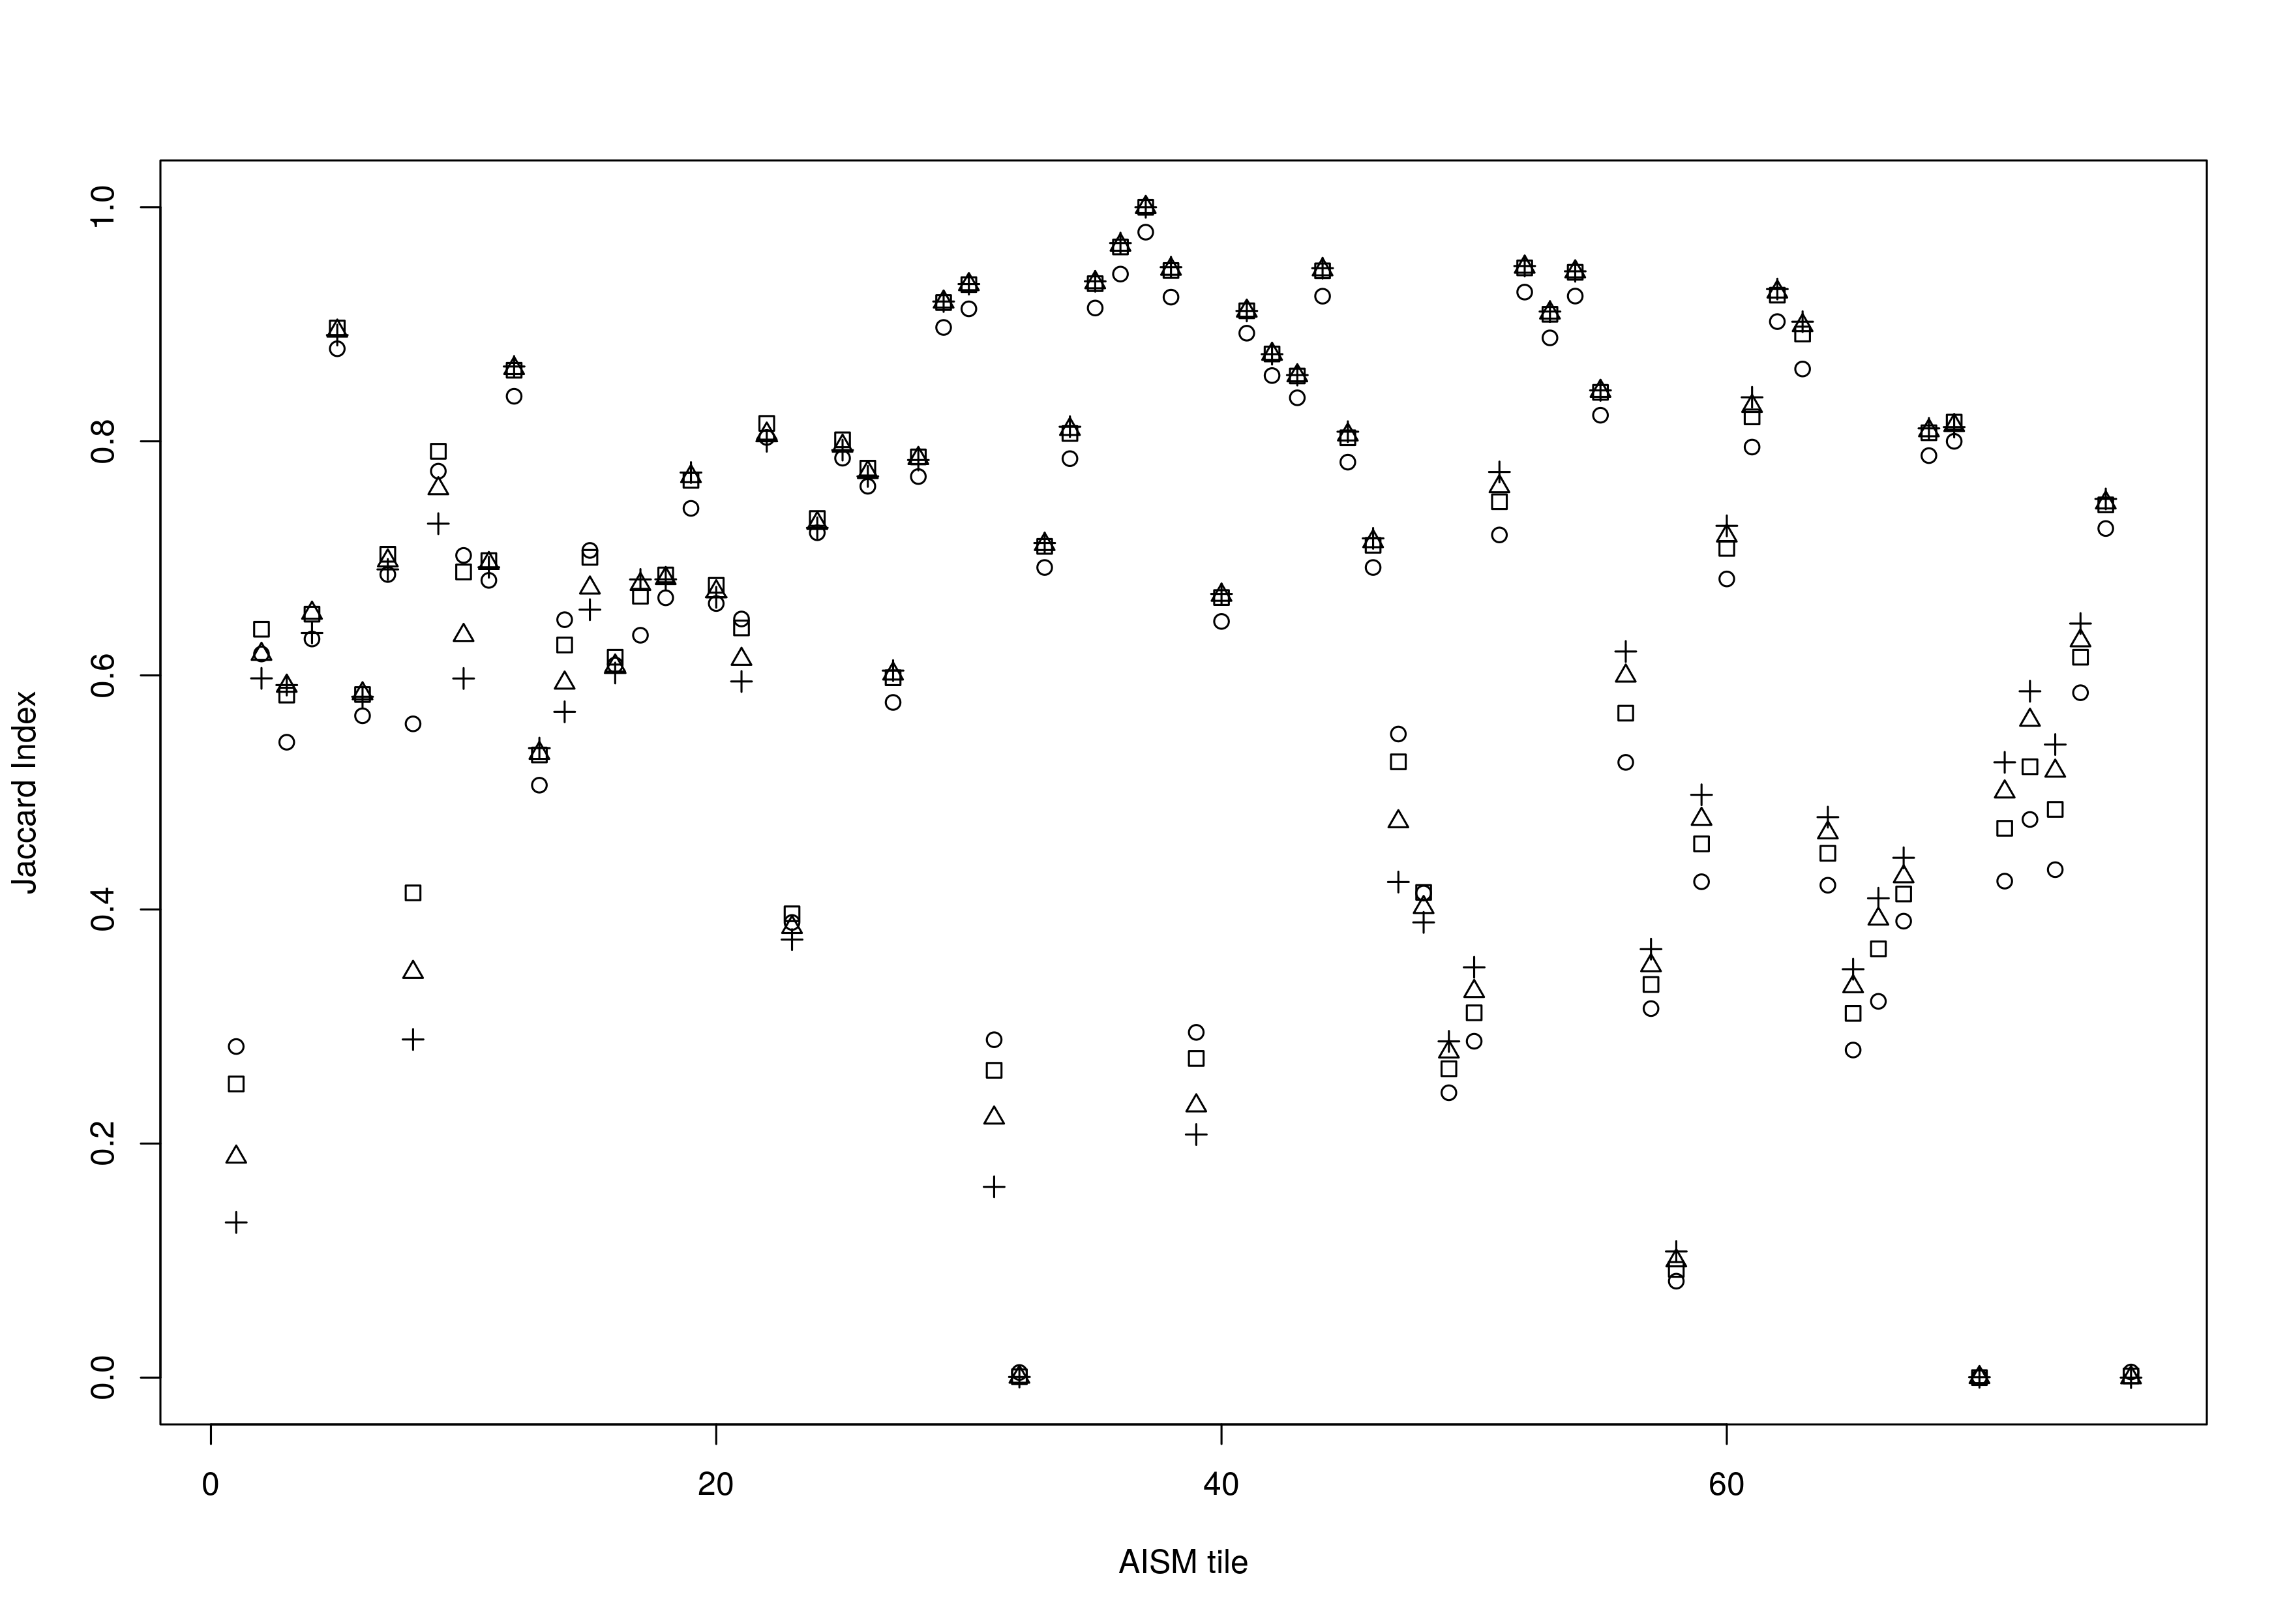
\includegraphics[scale=.65]{img/jaccard_tiles_americas}
				\caption[Jaccard Indexes for Latin American raster tiles]{\textbf{Jaccard Indexes for Latin American raster tiles:} Caption}
				\label{fig:jaccard_americas_appendix}
		\end{figure}
	\end{landscape}

	\begin{landscape}
		\begin{figure}[ht]
			\centering
			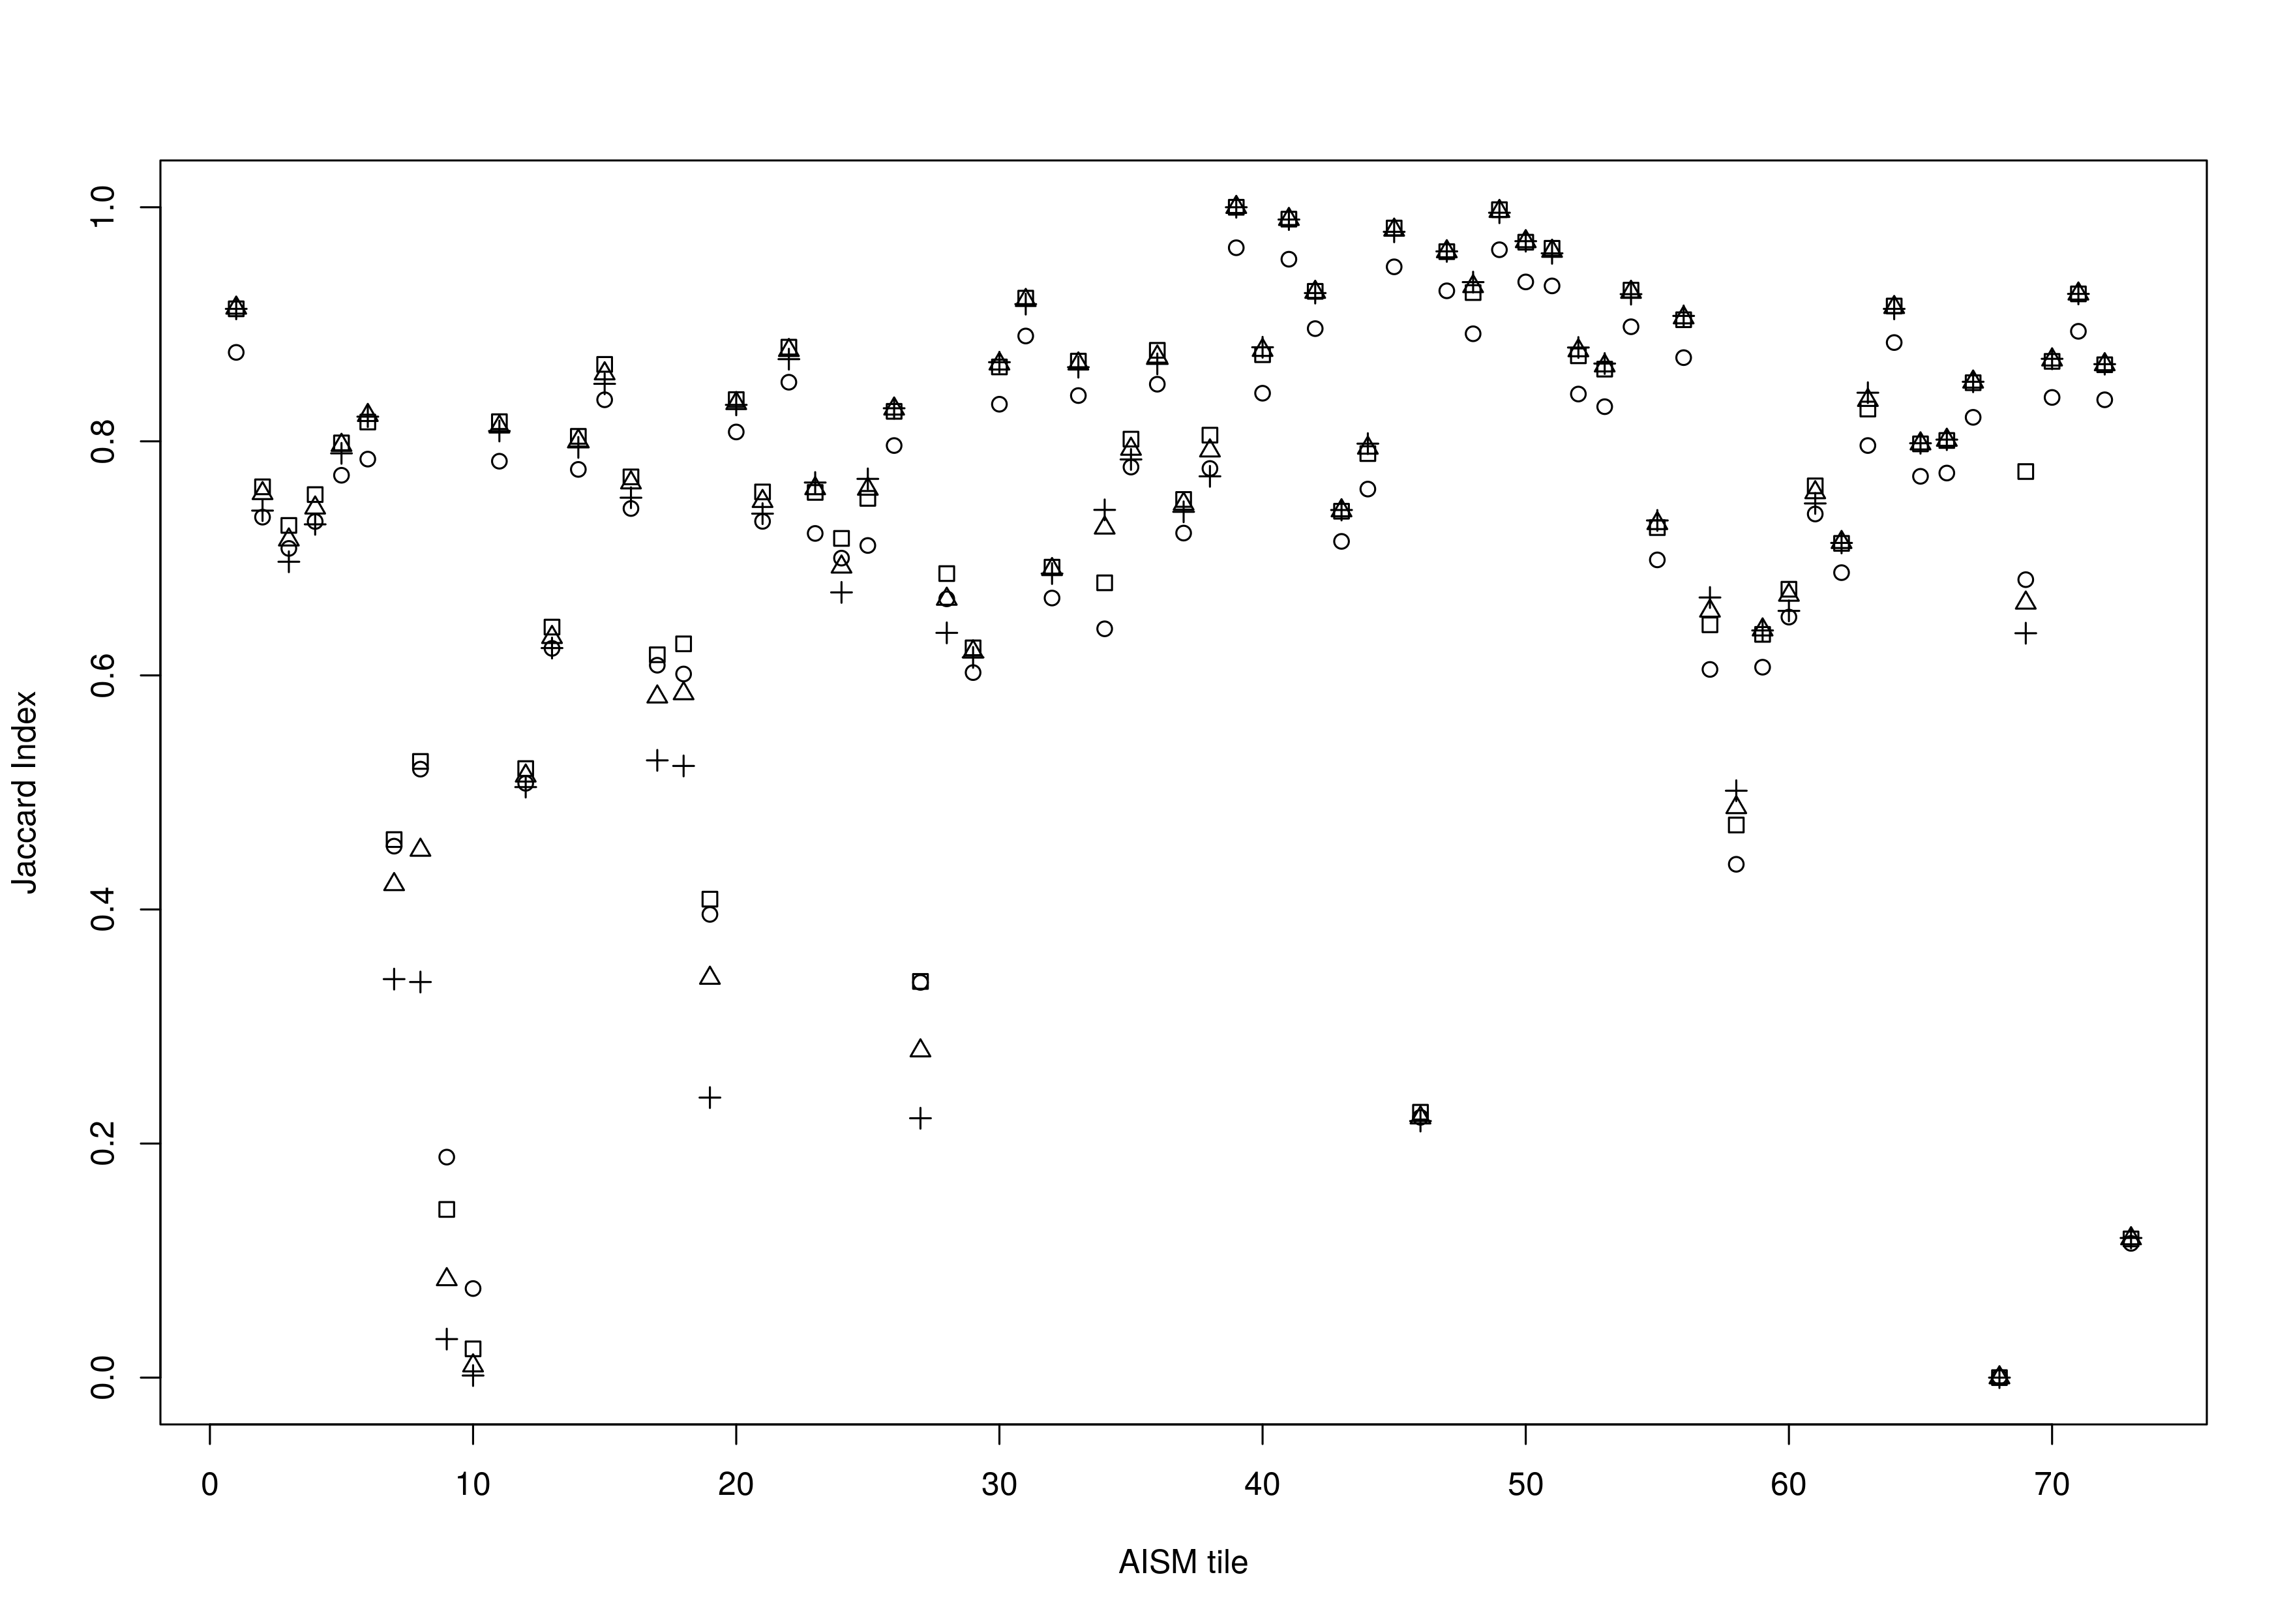
\includegraphics[scale=.65]{img/jaccard_tiles_asia}
			\caption[Jaccard Indexes for Asian/Australian raster tiles]{\textbf{Jaccard Indexes for Asian/Australian raster tiles:} Caption}
			\label{fig:jaccard_asia_appendix}
		\end{figure}
	\end{landscape}

	\begin{landscape}
		\begin{figure}[ht]
			\centering
			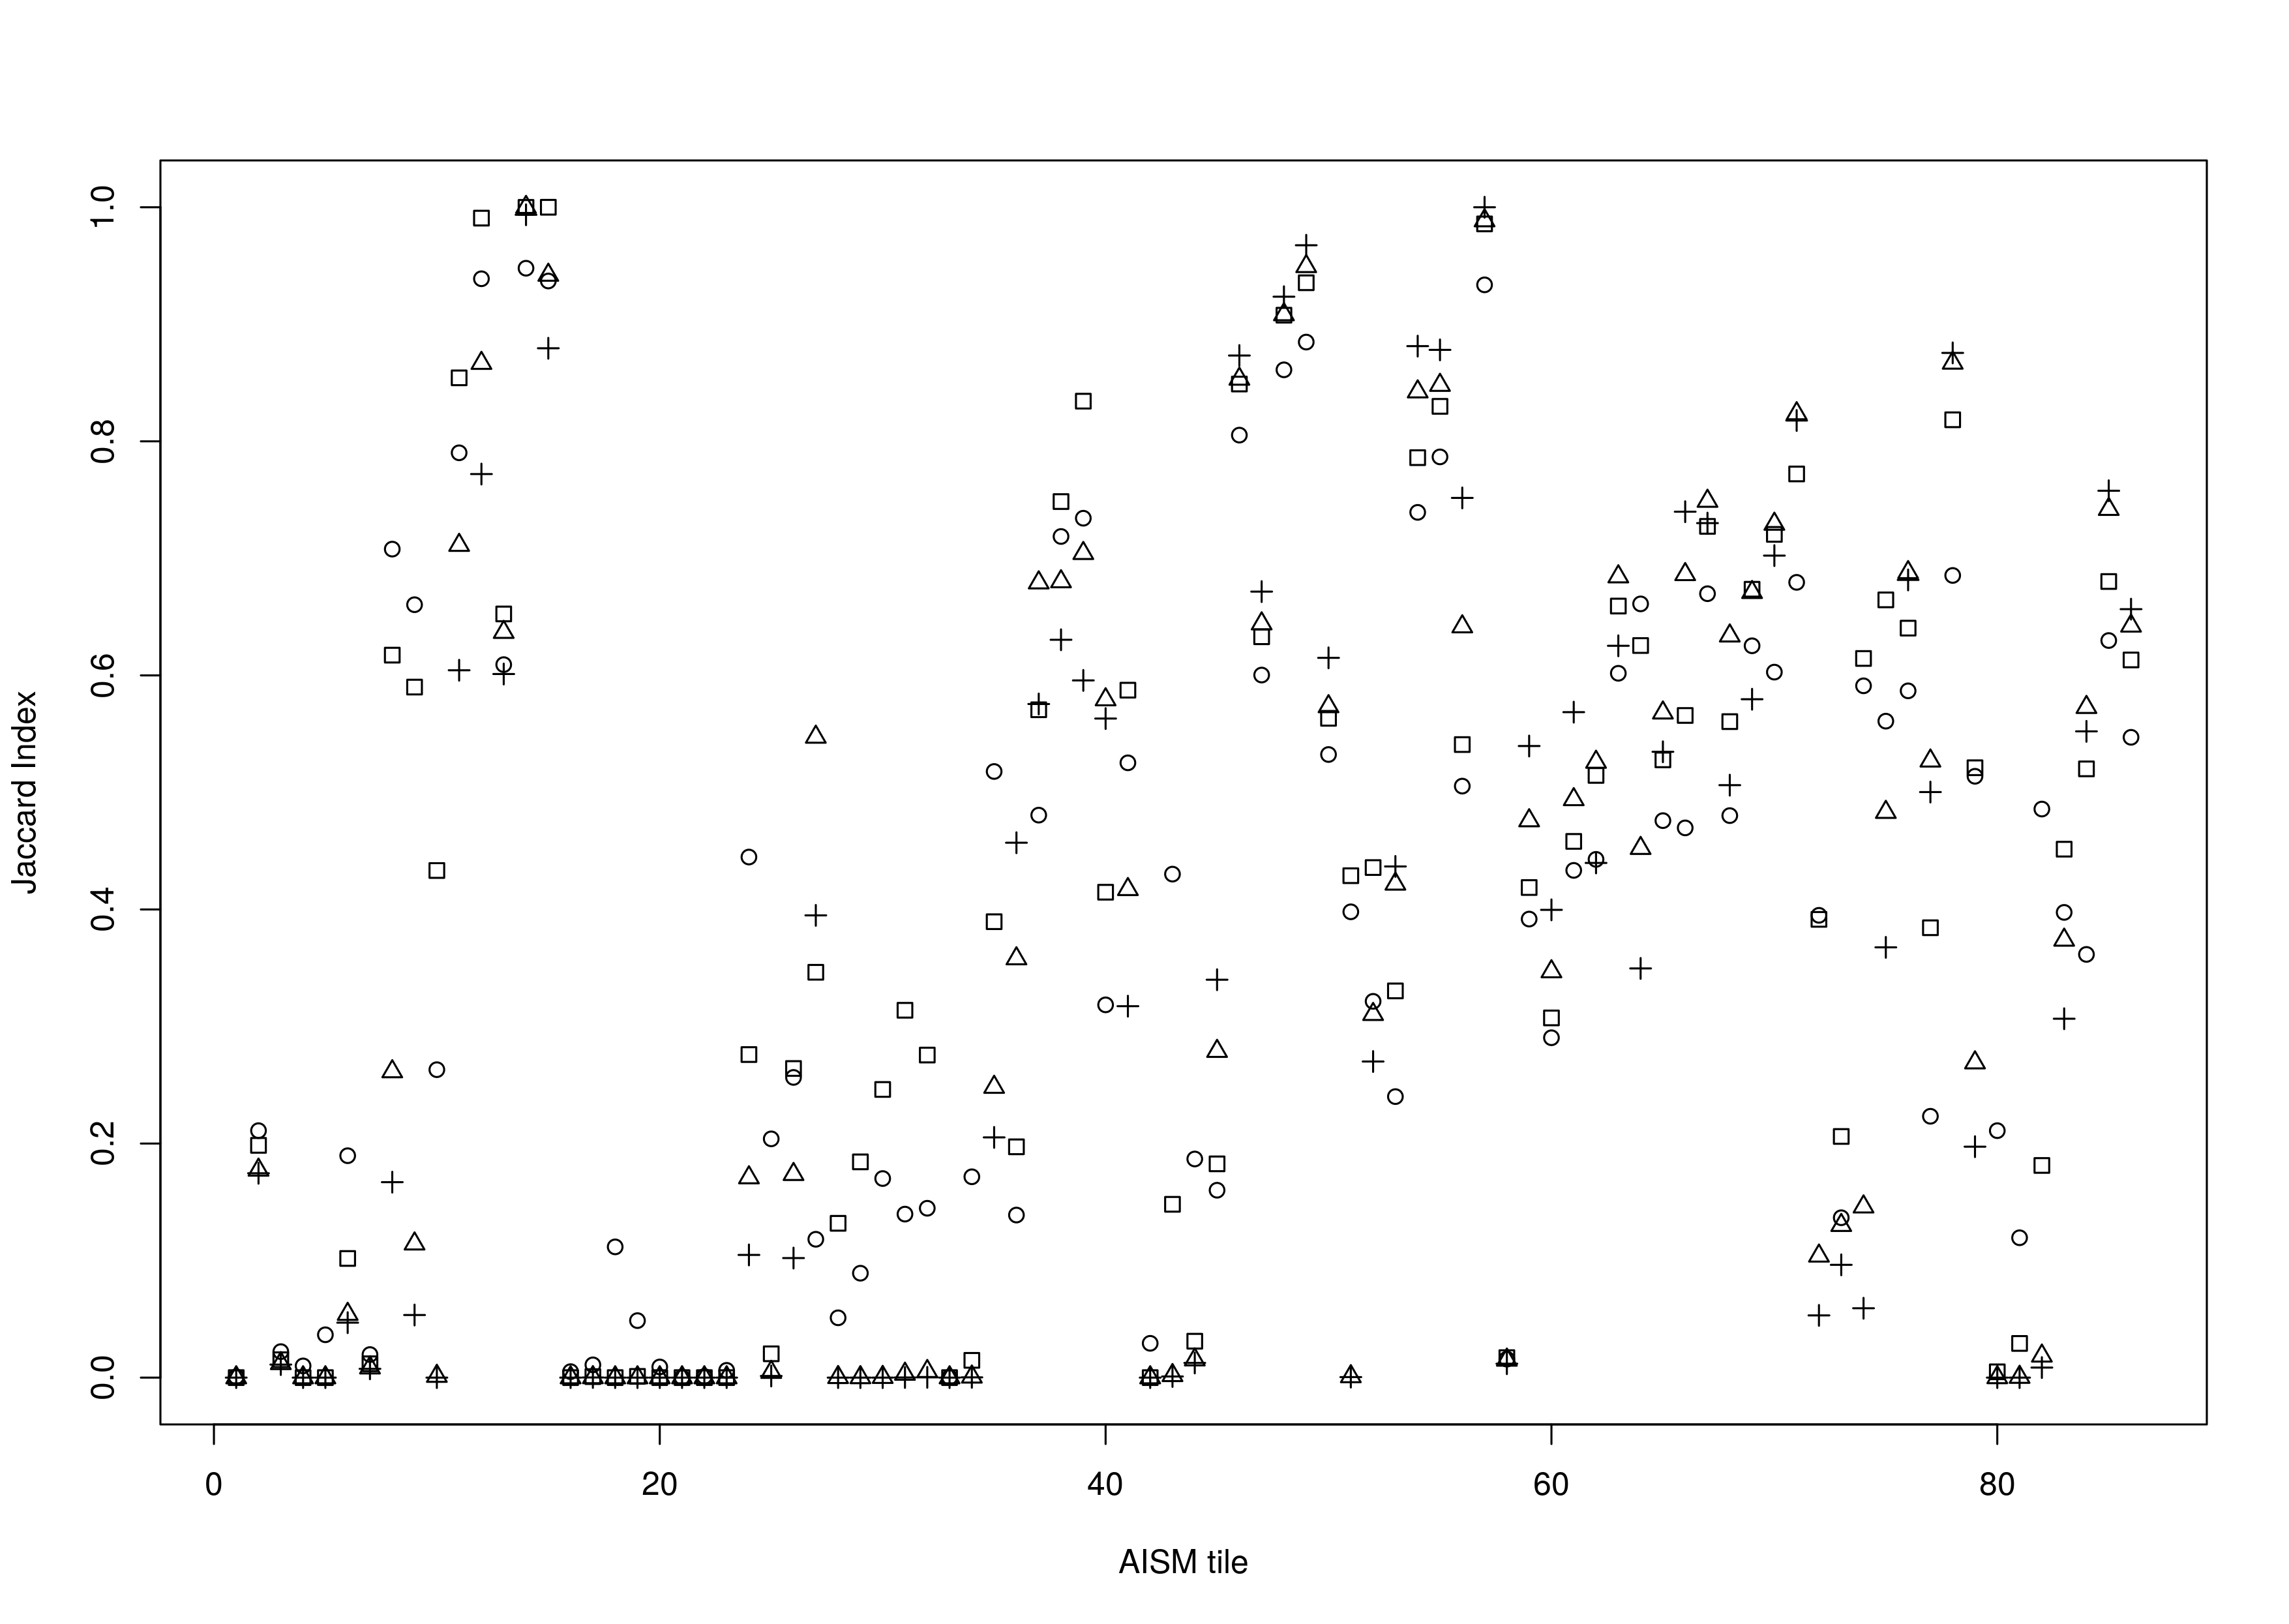
\includegraphics[scale=.65]{img/jaccard_tiles_africa}
			\caption[Jaccard Indexes for African raster tiles]{\textbf{Jaccard Indexes for African raster tiles:} Caption}
			\label{fig:jaccard_africa_appendix}
		\end{figure}
	\end{landscape}

\chapter{Proximate deforestation drivers}
\label{ch:appendix_c}
%TODO table: captions
	\begin{scriptsize}
	\begin{landscape}
		\begin{center}
			\begin{longtable}[ht]{lrrrrrrrrrr}
			\caption[Proximate drivers of deforestation for countries, continents, and globally]{\textbf{Proximate drivers of deforestation for countries, continents, and globally:}} \label{tab:proximate_driver}\\

			\hline
			Region&Cultivated&Forest&Regrowth&Grassland&Shrubland&Water&Artificial&Bareland&Total&Total$^\dagger$\\
			\hline
			\endfirsthead

			%\caption[]{continued}\\
			\hline
			Region&Cultivated&Forest&Regrowth&Grassland&Shrubland&Water&Artificial&Bareland&Total&Total$^\dagger$\\
			\hline
			\endhead

			\hline
			\endfoot

			%Latin America
			Argentina&5733.9 (65.8\%)&1380.6 (15.9\%)&147.9 (1.7\%)&461.8 (5.3\%)&718.7 (8.3\%)&230.8 (2.7\%)&32.8 (0.4\%)&2.0 (0.0\%)&8708.5&7097.1\\
			Bahamas&0.0 (0.0\%)&3.3 (41.2\%)&0.1 (1.3\%)&0.0 (0.0\%)&0.3 (3.8\%)&3.0 (37.5\%)&1.3 (16.3\%)&0.0 (0.0\%)&8.0&1.7\\
			Belize&212.2 (24.4\%)&113.0 (13.0\%)&155.5 (17.9\%)&308.9 (35.6\%)&54.5 (6.3\%)&12.7 (1.5\%)&11.1 (1.3\%)&0.0 (0.0\%)&867.9&742.2\\
			Bolivia&9288.2 (37.2\%)&5106.4 (20.5\%)&2428.1 (9.7\%)&5581.0 (22.4\%)&1825.1 (7.3\%)&590.8 (2.4\%)&108.3 (0.4\%)&19.5 (0.1\%)&24947.4&19250.2\\
			Brazil$^*$&56443.7 (19.1\%)&16433.7 (5.6\%)&34746.7 (11.8\%)&146802.9 (49.7\%)&35954.2 (12.2\%)&3832.4 (1.3\%)&738.8 (0.3\%)&209.0 (0.1\%)&295161.4&274895.3\\
			Chile$^*$&-&-&-&-&-&-&-&-&-&-\\
			Colombia&1297.9 (6.2\%)&5272.3 (25.2\%)&5177.2 (24.7\%)&6995.9 (33.4\%)&1593.1 (7.6\%)&573.6 (2.7\%)&26.0 (0.1\%)&9.7 (0.0\%)&20945.7&15099.8\\
			Costa Rica&307.4 (21.2\%)&536.8 (37.1\%)&178.5 (12.3\%)&397.4 (27.5\%)&11.0 (0.8\%)&7.0 (0.5\%)&9.0 (0.6\%)&0.1 (0.0\%)&1447.2&903.4\\
			Cuba&233.5 (17.6\%)&499.9 (37.7\%)&181.2 (13.7\%)&330.4 (24.9\%)&23.2 (1.8\%)&35.2 (2.7\%)&6.2 (0.5\%)&15.7 (1.2\%)&1325.3&790.2\\
			Dominican Republic&81.6 (5.4\%)&763.5 (50.5\%)&122.2 (8.1\%)&510.8 (33.8\%)&2.9 (0.2\%)&4.2 (0.3\%)&13.3 (0.9\%)&13.1 (0.9\%)&1511.6&743.9\\
			Ecuador&1143.9 (28.2\%)&1163.7 (28.7\%)&823.3 (20.3\%)&735.7 (18.1\%)&142.2 (3.5\%)&34.7 (0.9\%)&8.0 (0.2\%)&6.3 (0.2\%)&4057.8&2859.4\\
			El Salvador&58.1 (11.6\%)&28.2 (5.7\%)&6.2 (1.2\%)&390.9 (78.3\%)&8.5 (1.7\%)&1.6 (0.3\%)&5.6 (1.1\%)&0.0 (0.0\%)&499.1&469.3\\
			French Guiana&46.9 (14.7\%)&52.8 (16.5\%)&100.0 (31.2\%)&91.4 (28.6\%)&0.0 (0.0\%)&7.8 (2.4\%)&20.6 (6.4\%)&0.5 (0.2\%)&320.0&259.4\\
			Guatemala&1843.2 (23.9\%)&1172.6 (15.2\%)&924.2 (12.0\%)&2974.9 (38.6\%)&733.1 (9.5\%)&21.2 (0.3\%)&39.6 (0.5\%)&0.0 (0.0\%)&7708.8&6515.0\\
			Guyana&22.1 (3.1\%)&244.7 (34.3\%)&274.7 (38.5\%)&134.0 (18.8\%)&10.1 (1.4\%)&19.9 (2.8\%)&8.3 (1.2\%)&0.0 (0.0\%)&713.8&449.2\\
			Haiti&8.3 (3.9\%)&146.5 (69.3\%)&13.9 (6.6\%)&40.9 (19.3\%)&0.1 (0.0\%)&0.9 (0.4\%)&0.2 (0.1\%)&0.6 (0.3\%)&211.4&64.0\\
			Honduras&101.2 (2.5\%)&1200.1 (30.0\%)&487.9 (12.2\%)&2050.5 (51.2\%)&137.8 (3.4\%)&20.4 (0.5\%)&8.9 (0.2\%)&0.0 (0.0\%)&4006.8&2786.3\\
			Jamaica&7.2 (2.8\%)&127.7 (48.8\%)&25.5 (9.7\%)&82.4 (31.5\%)&0.0 (0.0\%)&1.9 (0.7\%)&16.7 (6.4\%)&0.3 (0.1\%)&261.7&132.1\\
			Mexico$^*$&3267.8 (18.7\%)&4857.8 (27.8\%)&3763.8 (21.5\%)&3950.6 (22.6\%)&1169.5 (6.7\%)&88.8 (0.5\%)&373.4 (2.1\%)&11.1 (0.1\%)&17482.8&12536.2\\
			Nicaragua&68.9 (0.9\%)&3405.0 (45.9\%)&1567.8 (21.2\%)&2268.8 (30.6\%)&78.3 (1.1\%)&19.9 (0.3\%)&2.5 (0.0\%)&0.0 (0.0\%)&7411.2&3986.3\\
			Panama&142.2 (6.3\%)&619.7 (27.6\%)&352.8 (15.7\%)&1019.7 (45.5\%)&70.8 (3.2\%)&22.3 (1.0\%)&13.5 (0.6\%)&0.4 (0.0\%)&2241.4&1599.4\\
			Paraguay$^*$&13718.0 (48.9\%)&6383.0 (22.8\%)&216.2 (0.8\%)&2480.2 (8.8\%)&5107.2 (18.2\%)&118.8 (0.4\%)&24.9 (0.1\%)&1.2 (0.0\%)&28049.5&21547.7\\
			Peru&780.4 (6.6\%)&2333.9 (19.8\%)&3394.0 (28.8\%)&2710.8 (23.0\%)&1230.9 (10.4\%)&1213.5 (10.3\%)&27.8 (0.2\%)&102.2 (0.9\%)&11793.5&8246.1\\
			Puerto Rico&4.1 (3.7\%)&56.4 (50.5\%)&10.2 (9.1\%)&30.7 (27.5\%)&0.0 (0.0\%)&0.4 (0.4\%)&8.8 (7.9\%)&1.0 (0.9\%)&111.6&54.8\\
			Suriname&36.7 (7.4\%)&132.2 (26.8\%)&167.5 (33.9\%)&108.5 (22.0\%)&0.0 (0.0\%)&40.8 (8.3\%)&8.2 (1.7\%)&0.0 (0.0\%)&493.9&320.9\\
			Venezuela&1082.3 (10.2\%)&2758.9 (26.1\%)&1644.0 (15.5\%)&3382.4 (32.0\%)&1388.8 (13.1\%)&267.4 (2.5\%)&47.7 (0.5\%)&12.7 (0.1\%)&10584.2&7557.9\\\hline
			Latin America&95929.7 (21.3\%)&54792.7 (12.2\%)&56909.4 (12.6\%)&183841.5 (40.8\%)&50260.3 (11.1\%)&7170.0 (1.6\%)&1561.5 (0.3\%)&405.4 (0.1\%)&450870.5&388907.8\\\hline

			%Africa
			Algeria$^*$&-&-&-&-&-&-&-&-&-&-\\
			Angola&4818.6 (32.7\%)&697.8 (4.7\%)&452.5 (3.1\%)&8065.9 (54.7\%)&371.2 (2.5\%)&90.9 (0.6\%)&226.5 (1.5\%)&10.9 (0.1\%)&14734.3&13945.6\\
			Benin&1518.7 (58.2\%)&200.6 (7.7\%)&45.1 (1.7\%)&74.6 (2.9\%)&762.5 (29.2\%)&0.5 (0.0\%)&5.6 (0.2\%)&0.0 (0.0\%)&2607.6&2406.5\\
			Botswana$^*$&9.4 (17.9\%)&2.1 (4.0\%)&0.0 (0.0\%)&26.4 (50.2\%)&3.6 (6.8\%)&9.9 (18.8\%)&1.2 (2.3\%)&0.0 (0.0\%)&52.6&40.6\\
			Burkina Faso&510.9 (29.4\%)&4.6 (0.3\%)&0.0 (0.0\%)&1190.0 (68.5\%)&31.7 (1.8\%)&0.3 (0.0\%)&0.1 (0.0\%)&0.7 (0.0\%)&1738.3&1733.4\\
			Burundi&49.7 (30.6\%)&6.3 (3.9\%)&3.6 (2.2\%)&98.8 (60.9\%)&2.0 (1.2\%)&0.5 (0.3\%)&1.3 (0.8\%)&0.0 (0.0\%)&162.2&155.4\\
			Cameroon&337.8 (8.5\%)&938.2 (23.6\%)&717.2 (18.1\%)&1838.8 (46.3\%)&14.4 (0.4\%)&34.6 (0.9\%)&68.6 (1.7\%)&21.6 (0.5\%)&3971.2&2998.4\\
			C. African Rep.&707.3 (18.3\%)&217.1 (5.6\%)&328.4 (8.5\%)&2470.2 (64.1\%)&118.6 (3.1\%)&3.3 (0.1\%)&9.8 (0.3\%)&0.6 (0.0\%)&3855.3&3634.9\\
			Chad&1454.7 (54.7\%)&1.8 (0.1\%)&0.1 (0.0\%)&1037.5 (39.0\%)&142.2 (5.4\%)&15.9 (0.6\%)&3.1 (0.1\%)&2.4 (0.1\%)&2657.7&2640.0\\
			Congo&107.8 (4.9\%)&406.0 (18.4\%)&591.8 (26.8\%)&968.0 (43.8\%)&0.3 (0.0\%)&109.7 (5.0\%)&25.8 (1.2\%)&0.1 (0.0\%)&2209.5&1693.8\\
			DR Congo&4771.8 (9.4\%)&3518.2 (6.9\%)&13508.7 (26.6\%)&26400.4 (52.0\%)&508.2 (1.0\%)&1736.9 (3.4\%)&314.7 (0.6\%)&0.1 (0.0\%)&50759.0&45503.9\\
			Djibouti&-&-&-&-&-&-&-&-&-&-\\
			Egypt$^*$&-&-&-&-&-&-&-&-&-&-\\
			Equatorial Guinea&0.0 (0.0\%)&77.2 (28.7\%)&77.7 (28.9\%)&72.6 (27.0\%)&1.3 (0.5\%)&1.3 (0.5\%)&38.5 (14.3\%)&0.0 (0.0\%)&268.6&190.1\\
			Eritrea&0.0 (0.0\%)&0.0 (0.0\%)&0.0 (0.0\%)&0.1 (100.0\%)&0.0 (0.0\%)&0.0 (0.0\%)&0.0 (0.0\%)&0.0 (0.0\%)&0.1&0.1\\
			Ethiopia&356.8 (16.1\%)&296.9 (13.4\%)&137.2 (6.2\%)&1321.6 (59.5\%)&92.3 (4.2\%)&4.5 (0.2\%)&3.9 (0.2\%)&6.6 (0.3\%)&2219.8&1918.4\\
			Gabon&1.4 (0.1\%)&528.7 (32.9\%)&664.1 (41.3\%)&362.7 (22.5\%)&0.0 (0.0\%)&22.9 (1.4\%)&24.9 (1.5\%)&3.9 (0.2\%)&1608.6&1057.0\\
			Gambia&35.6 (29.1\%)&0.0 (0.0\%)&0.0 (0.0\%)&63.5 (51.9\%)&19.8 (16.2\%)&0.1 (0.1\%)&3.4 (2.8\%)&0.0 (0.0\%)&122.4&122.3\\
			Ghana&319.1 (6.8\%)&525.3 (11.1\%)&1523.7 (32.3\%)&1990.8 (42.2\%)&235.5 (5.0\%)&27.6 (0.6\%)&95.0 (2.0\%)&0.0 (0.0\%)&4717.0&4164.1\\
			Guinea&261.3 (8.2\%)&61.2 (1.9\%)&118.0 (3.7\%)&2296.7 (72.4\%)&419.2 (13.2\%)&3.3 (0.1\%)&11.4 (0.4\%)&2.1 (0.1\%)&3173.2&3108.7\\
			Guinea Bissau&136.7 (24.5\%)&2.3 (0.4\%)&15.5 (2.8\%)&181.5 (32.5\%)&216.6 (38.8\%)&1.2 (0.2\%)&3.9 (0.7\%)&0.0 (0.0\%)&557.7&554.2\\
			Ivory Coast&1636.4 (12.5\%)&2619.8 (20.0\%)&2515.1 (19.2\%)&6147.4 (46.9\%)&81.7 (0.6\%)&34.0 (0.3\%)&69.1 (0.5\%)&0.7 (0.0\%)&13104.2&10450.4\\
			Kenya&1178.9 (48.1\%)&118.8 (4.9\%)&213.6 (8.7\%)&832.7 (34.0\%)&85.7 (3.5\%)&13.7 (0.6\%)&4.2 (0.2\%)&1.6 (0.1\%)&2449.2&2316.7\\
			Liberia&8.1 (0.2\%)&395.4 (12.0\%)&1863.5 (56.6\%)&986.7 (30.0\%)&3.5 (0.1\%)&2.2 (0.1\%)&30.7 (0.9\%)&0.0 (0.0\%)&3290.1&2892.5\\
			Libya$^*$&-&-&-&-&-&-&-&-&-&-\\
			Madagascar&197.1 (1.6\%)&667.1 (5.3\%)&5126.0 (40.6\%)&5627.5 (44.6\%)&957.9 (7.6\%)&43.5 (0.3\%)&1.5 (0.0\%)&0.1 (0.0\%)&12620.7&11910.1\\
			Malawi&457.8 (40.0\%)&185.4 (16.2\%)&83.6 (7.3\%)&398.3 (34.8\%)&8.3 (0.7\%)&1.9 (0.2\%)&4.6 (0.4\%)&4.7 (0.4\%)&1144.6&957.3\\
			Mali&480.6 (39.4\%)&1.0 (0.1\%)&0.0 (0.0\%)&708.7 (58.1\%)&25.6 (2.1\%)&0.6 (0.0\%)&2.9 (0.2\%)&0.3 (0.0\%)&1219.7&1218.1\\
			Mauritania&0.0 (0.0\%)&0.0 (0.0\%)&0.0 (0.0\%)&0.2 (33.3\%)&0.4 (66.7\%)&0.0 (0.0\%)&0.0 (0.0\%)&0.0 (0.0\%)&0.6&0.6\\
			Morocco$^*$&-&-&-&-&-&-&-&-&-&-\\
			Mozambique$^*$&6419.1 (32.7\%)&1527.7 (7.8\%)&1967.4 (10.0\%)&8959.4 (45.6\%)&664.8 (3.4\%)&49.2 (0.3\%)&37.0 (0.2\%)&17.8 (0.1\%)&19642.4&18065.5\\
			Namibia$^*$&46.1 (38.0\%)&6.8 (5.6\%)&0.0 (0.0\%)&59.9 (49.4\%)&5.1 (4.2\%)&2.1 (1.7\%)&1.0 (0.8\%)&0.2 (0.2\%)&121.2&112.3\\
			Niger&0.0 (0.0\%)&0.0 (0.0\%)&0.0 (0.0\%)&0.9 (10.3\%)&0.0 (0.0\%)&7.8 (89.7\%)&0.0 (0.0\%)&0.0 (0.0\%)&8.7&0.9\\
			Nigeria&2392.5 (34.4\%)&1462.3 (21.0\%)&452.3 (6.5\%)&1754.3 (25.2\%)&689.8 (9.9\%)&24.4 (0.4\%)&122.3 (1.8\%)&63.6 (0.9\%)&6961.5&5474.8\\
			Rwanda&65.9 (42.7\%)&18.2 (11.8\%)&16.3 (10.6\%)&46.3 (30.0\%)&5.8 (3.8\%)&0.6 (0.4\%)&1.2 (0.8\%)&0.0 (0.0\%)&154.3&135.5\\
			Senegal&221.4 (30.0\%)&0.3 (0.0\%)&0.1 (0.0\%)&401.5 (54.4\%)&112.2 (15.2\%)&0.7 (0.1\%)&1.6 (0.2\%)&0.0 (0.0\%)&737.8&736.8\\
			Sierra Leone&11.1 (0.7\%)&167.3 (10.1\%)&455.9 (27.5\%)&995.0 (60.1\%)&6.1 (0.4\%)&3.2 (0.2\%)&16.3 (1.0\%)&0.0 (0.0\%)&1654.9&1484.4\\
			Somalia&7.2 (11.0\%)&10.0 (15.3\%)&0.1 (0.2\%)&0.9 (1.4\%)&46.0 (70.6\%)&0.9 (1.4\%)&0.1 (0.2\%)&0.0 (0.0\%)&65.2&54.3\\
			Somaliland&0.0 (0.0\%)&0.2 (66.7\%)&0.0 (0.0\%)&0.0 (0.0\%)&0.1 (33.3\%)&0.0 (0.0\%)&0.0 (0.0\%)&0.0 (0.0\%)&0.3&0.1\\
			South Africa$^*$&47.5 (8.3\%)&2.9 (0.5\%)&319.2 (56.1\%)&190.8 (33.5\%)&2.8 (0.5\%)&1.6 (0.3\%)&4.2 (0.7\%)&0.3 (0.1\%)&569.3&564.8\\
			South Sudan&291.4 (21.4\%)&64.7 (4.7\%)&15.1 (1.1\%)&792.5 (58.1\%)&161.9 (11.9\%)&30.5 (2.2\%)&8.2 (0.6\%)&0.3 (0.0\%)&1364.6&1269.4\\
			Sudan&1.2 (3.7\%)&0.2 (0.6\%)&0.0 (0.0\%)&22.5 (69.7\%)&7.7 (23.8\%)&0.6 (1.9\%)&0.0 (0.0\%)&0.1 (0.3\%)&32.3&31.5\\
			Tanzania&6677.4 (42.1\%)&1013.2 (6.4\%)&1397.1 (8.8\%)&6436.0 (40.6\%)&247.6 (1.6\%)&38.0 (0.2\%)&28.6 (0.2\%)&7.2 (0.0\%)&15845.1&14793.9\\
			Togo&345.5 (48.2\%)&65.1 (9.1\%)&8.4 (1.2\%)&23.8 (3.3\%)&270.0 (37.7\%)&2.1 (0.3\%)&1.7 (0.2\%)&0.0 (0.0\%)&716.6&649.4\\
			Uganda&777.8 (27.7\%)&75.7 (2.7\%)&153.3 (5.5\%)&1772.0 (63.1\%)&9.6 (0.3\%)&15.0 (0.5\%)&4.7 (0.2\%)&0.0 (0.0\%)&2808.1&2717.4\\
			West Sahara&-&-&-&-&-&-&-&-&-&-\\
			Zambia&5966.6 (53.5\%)&1111.0 (10.0\%)&110.1 (1.0\%)&3614.2 (32.4\%)&216.0 (1.9\%)&70.0 (0.6\%)&54.5 (0.5\%)&0.0 (0.0\%)&11142.4&9961.4\\
			Zimbabwe&1662.3 (55.6\%)&95.7 (3.2\%)&100.1 (3.3\%)&1069.8 (35.8\%)&51.5 (1.7\%)&4.0 (0.1\%)&6.5 (0.2\%)&0.1 (0.0\%)&2990.0&2890.3\\\hline
			Africa&44289.5 (22.8\%)&17093.1 (8.8\%)&32980.8 (17.0\%)&89301.4 (46.0\%)&6599.5 (3.4\%)&2410.0 (1.2\%)&1238.6 (0.6\%)&146.0 (0.1\%)&194058.9&174555.8\\\hline

			%Asia/Australia
			Australia$^*$&0.0 (0.0\%)&1.0 (17.2\%)&0.6 (10.3\%)&0.8 (13.8\%)&2.9 (50.0\%)&0.2 (3.4\%)&0.0 (0.0\%)&0.3 (5.2\%)&5.8&4.6\\
			Bangladesh$^*$&86.5 (19.4\%)&216.9 (48.7\%)&85.0 (19.1\%)&36.9 (8.3\%)&8.2 (1.8\%)&2.0 (0.4\%)&8.7 (2.0\%)&1.1 (0.2\%)&445.3&226.4\\
			Brunei&3.4 (1.3\%)&24.4 (9.0\%)&204.2 (75.3\%)&17.5 (6.5\%)&0.0 (0.0\%)&2.9 (1.1\%)&18.7 (6.9\%)&0.0 (0.0\%)&271.1&243.8\\
			Cambodia&3014.8 (34.0\%)&2279.7 (25.7\%)&2200.1 (24.8\%)&1027.9 (11.6\%)&0.0 (0.0\%)&327.9 (3.7\%)&13.3 (0.2\%)&0.0 (0.0\%)&8863.7&6256.1\\
			China$^*$&3193.3 (15.4\%)&3009.9 (14.5\%)&10801.1 (52.0\%)&2710.0 (13.0\%)&940.1 (4.5\%)&57.8 (0.3\%)&59.8 (0.3\%)&0.2 (0.0\%)&20772.2&17704.5\\
			East Timor&4.0 (3.0\%)&55.8 (41.3\%)&43.3 (32.0\%)&29.1 (21.5\%)&0.0 (0.0\%)&1.9 (1.4\%)&0.0 (0.0\%)&1.1 (0.8\%)&135.2&77.5\\
			India$^*$&658.8 (23.4\%)&976.9 (34.7\%)&716.9 (25.5\%)&290.5 (10.3\%)&142.4 (5.1\%)&8.6 (0.3\%)&20.7 (0.7\%)&1.1 (0.0\%)&2815.9&1830.4\\
			Indonesia&17415.1 (15.4\%)&11227.1 (9.9\%)&77352.2 (68.6\%)&5209.1 (4.6\%)&0.0 (0.0\%)&1312.1 (1.2\%)&303.0 (0.3\%)&17.2 (0.0\%)&112835.8&100296.6\\
			Laos&1390.7 (14.8\%)&1078.2 (11.5\%)&5352.5 (57.0\%)&1537.3 (16.4\%)&9.7 (0.1\%)&11.4 (0.1\%)&4.3 (0.0\%)&6.4 (0.1\%)&9390.5&8300.9\\
			Malaysia&2722.1 (7.5\%)&3238.3 (8.9\%)&29001.4 (79.4\%)&963.6 (2.6\%)&0.0 (0.0\%)&249.8 (0.7\%)&359.4 (1.0\%)&0.3 (0.0\%)&36534.9&33046.8\\
			Myanmar$^*$&2430.4 (24.5\%)&2406.7 (24.3\%)&3622.2 (36.6\%)&904.1 (9.1\%)&383.8 (3.9\%)&140.0 (1.4\%)&21.1 (0.2\%)&0.1 (0.0\%)&9908.4&7361.7\\
			Pakistan&0.1 (50.0\%)&0.0 (0.0\%)&0.0 (0.0\%)&0.0 (0.0\%)&0.0 (0.0\%)&0.1 (50.0\%)&0.0 (0.0\%)&0.0 (0.0\%)&0.2&0.1\\
			Papua New Guinea&177.6 (3.8\%)&1264.6 (26.8\%)&2630.7 (55.7\%)&318.8 (6.8\%)&188.1 (4.0\%)&115.8 (2.5\%)&14.8 (0.3\%)&10.9 (0.2\%)&4721.3&3340.9\\
			Philippines&550.9 (12.4\%)&1247.3 (28.1\%)&2178.2 (49.0\%)&423.3 (9.5\%)&0.1 (0.0\%)&37.4 (0.8\%)&7.0 (0.2\%)&0.2 (0.0\%)&4444.4&3159.7\\
			Saudi Arabia$^*$&-&-&-&-&-&-&-&-&-&-\\
			Solomon Island&0.0 (0.0\%)&84.6 (36.2\%)&101.2 (43.2\%)&19.6 (8.4\%)&27.4 (11.7\%)&1.0 (0.4\%)&0.1 (0.0\%)&0.1 (0.0\%)&234.0&148.4\\
			Sri Lanka&274.4 (42.0\%)&213.5 (32.7\%)&108.3 (16.6\%)&42.4 (6.5\%)&0.0 (0.0\%)&5.2 (0.8\%)&9.3 (1.4\%)&0.3 (0.0\%)&653.4&434.7\\
			Taiwan$^*$&24.6 (11.2\%)&110.4 (50.3\%)&37.8 (17.2\%)&45.2 (20.6\%)&0.0 (0.0\%)&0.7 (0.3\%)&0.8 (0.4\%)&0.0 (0.0\%)&219.5&108.4\\
			Thailand&1943.9 (22.6\%)&1989.6 (23.1\%)&3463.3 (40.2\%)&1090.8 (12.7\%)&0.0 (0.0\%)&99.2 (1.2\%)&29.5 (0.3\%)&0.0 (0.0\%)&8616.3&6527.5\\
			Vanuatu&0.0 (0.0\%)&0.1 (100.0\%)&0.0 (0.0\%)&0.0 (0.0\%)&0.0 (0.0\%)&0.0 (0.0\%)&0.0 (0.0\%)&0.0 (0.0\%)&0.1&0.0\\
			Vietnam&2928.7 (32.8\%)&1102.2 (12.3\%)&2754.5 (30.8\%)&1635.7 (18.3\%)&443.5 (5.0\%)&57.9 (0.6\%)&19.5 (0.2\%)&0.2 (0.0\%)&8942.2&7782.1\\
			Yemen$^*$&-&-&-&-&-&-&-&-&-&-\\\hline
			Asia/Australia&36819.3 (16.0\%)&30527.2 (13.3\%)&140653.5 (61.2\%)&16302.6 (7.1\%)&2146.2 (0.9\%)&2431.9 (1.1\%)&890.0 (0.4\%)&39.5 (0.0\%)&229810.2&196851.1\\\hline

			%Global
			Global&177038.5 (20.2\%)&102412.9 (11.7\%)&230543.7 (26.4\%)&289445.5 (33.1\%)&59005.9 (6.7\%)&12011.9 (1.4\%)&3690.1 (0.4\%)&590.9 (0.1\%)&874739.6&\\
			\end{longtable}
		\end{center}
	\end{landscape}
\end{scriptsize}